\documentclass[conference]{IEEEtran}
\IEEEoverridecommandlockouts
% The preceding line is only needed to identify funding in the first footnote. If that is unneeded, please comment it out.
\usepackage{cite}
\usepackage{amsmath,amssymb,amsfonts}
\usepackage{algorithmic}
\usepackage{graphicx}
\usepackage{textcomp}
\usepackage{xcolor}
\usepackage{booktabs}
\usepackage{csvsimple}
\usepackage{float}
\usepackage{caption}
\usepackage{tabularx}
\def\BibTeX{{\rm B\kern-.05em{\sc i\kern-.025em b}\kern-.08em
    T\kern-.1667em\lower.7ex\hbox{E}\kern-.125emX}}
\begin{document}

\title{Performance comparison between simple RNNs*\\
{\footnotesize \textsuperscript{*}Note: Sub-titles are not captured in Xplore and
should not be used}
\thanks{Identify applicable funding agency here. If none, delete this.}
}

\author{\IEEEauthorblockN{1\textsuperscript{st} Christopher John Klopper}
\IEEEauthorblockA{\textit{Department of Data Science} \\
\textit{Stellenbosch University}\\
Stellenbosch, South Africa\\
26090074@sun.ac.za}

}

\maketitle

\begin{abstract}
% TODO
\end{abstract}

\begin{IEEEkeywords}
component, formatting, style, styling, insert
\end{IEEEkeywords}

\section{Introduction}

% TODO

This paper will mathematically define the structures of the Elman, Jordan and multi-recurrent simple neural networks. It will also showcase how different data sets with different sizes and data distribution qualities impact the performance of the models and how to mitigate under-fitting and over-fitting. Also covered will be a motivated choice on which architecture to select for each of the data sets considered.

\section{Pre-processing and description of datasets}

Some of the datasets contained data issues which needed to be dealt with before training the models.

\subsection{Dataset 1: Apple Stock Data}

Pre-processing included converting the string date into a DateTime format. Converting strings to float and int datatypes, where appropriate. Renaming columns for convenience. The Closing\_Price column was a string type with a '\$' sign pre-pended to the front. This was removed and the feature was converted to a float value since the RNN requires all features to be numerical. The Year, Month, Day and Weekday features were extracted from the DateTime and converted into two dimensions using sine and cosine transformations. This was done because the RNN requires all features to be numerical. Volume, Open, High, Low, Date, Year, Month, Day, Weekday features were dropped since we are only interested in predicting the closing price for the day and some of the features were redundant. Here are the summary statistics before pre-processing:

\begin{table}[htbp]
	\caption{Summary statistics for Apple stock data}
	\resizebox{\columnwidth}{!}{
		\csvautobooktabular{../csv-descriptions/apple-raw-data-description.csv}
	}
	\label{tab:apple-stats}
\end{table}

The Apple stock data is non-stationary. The Apple stock data is a regression problem. The distributions were inspected using bar plots and no outliers or noise was found.

\subsection{Dataset 2: Cape Town weather data}

The data was sourced from Kaggle (https://www.kaggle.com/datasets/muthuj7/weather-dataset). For experimentation almost all features except the time and average temperature for the day was removed. Relevant features were extracted from the date (Year, Month, DayOfWeek, DayOfYear, WeekOfYear) and converted into two dimensions using sine and cosine transformations.

\begin{table}[htbp]
	\centering
	\small
	\caption{Summary statistics for Cape Town weather data}
	\csvautobooktabular{../csv-descriptions/weather-stats.csv}
	\label{tab:ct}
\end{table}


The Cape Town weather data is non-stationary. The Cape Town weather data is a regression problem. The distributions were inspected and no outliers or noise was found.
 
\subsection{Dataset 3: Air quality data}

This data set was obtained from the UCI Machine Learning repository (https://archive.ics.uci.edu/dataset/360/air+quality), more information on the data set can be obtained there. For this experimentation, we will try and predict the PT08.S3(NOx) feature of the data set.

There were some empty rows and columns in the data set which were dropped. The HourOfDay, DayOfWeek and Month feature was extracted from the dates. The Year feature was not extracted as the data only spanned two years and the years did not provide any information. These features were converted to two dimensions using sine and cosine transformations. The ',' character was replaced with the '.' character in order to ensure that floats were correctly parsed. There were errors with the sensors where readings were less then or equal to 0, fill forward was used to replace these errors. PT08.S1(CO), C6H6(GT), PT08.S2(NMHC) were highly correlated with another feature so these features were dropped. The target feature also had these less or equal to 0 errors so all observations where the target feature had this error was dropped.

\begin{table}[htbp]
	\centering
	\caption{Summary statistics for Air Quality data}
	\resizebox{\columnwidth}{!}{
		\csvautobooktabular{../csv-descriptions/airquality-stats.csv}
	}
	\label{tab:aq-stats}
\end{table}


The Air quality data is stationary. The Air quality data is a regression problem. The distributions were inspected and no outliers or noise were found. These outliers were not reading/sensor errors but part of natural distribution of dataset. 
\subsection{Dataset 4: Property price data}



\subsection{Dataset 5: }

\section{Background: Time series cross-validation}

\subsection{Time-series-split}

Creates folds where the observations of the validation set are always after the observations of the test set. The start of each fold is the beginning of the dataset. This allows for more splits, but creates leakage from future data to the model. The \texttt{sklearn.model\_selection.TimeSeriesSplit} time series split method was used during cross validation of models. If cross-validation is mentioned in this paper it refers to Time-series-split cross-validation.

\subsection{Blocked cross-validation}

Works the same as time-series split but with added margins. One added between training and validation set. This is due to the correlation between observations at the end of the training set and beginning of validation set being very high, allowing the model to cheat a little bit. The second margin is added between the folds themselves, to prevent models from learning patterns from one fold iteration to the next. This allows for more splits and solves the data leakage issue but comes with the cost of increased computational requirements.

\section{Background: RNN network architectures}

This section covers current literature on the different RNN architectures experimented with in this paper.

\subsection{Elman and Jordan recurrent neural network}

Both the Elman and Jordan RNNs are three layer networks (input, hidden and output layer) with the Jordan RNN having an additional state vector (known as context units). The following notation is defined:

\begin{enumerate}
	\item $a,b,c,d,e,f,g \in \mathbb{Z}_{>0}$: A positive non-zero integer
	
	\item $x_t \in \mathbb{R}^a$: Input layer vector at time t
	\item $h_t \in \mathbb{R}^b$: Hidden layer vector at time t
	\item $y_t \in \mathbb{R}^c$: Output layer vector at time t
	
	\item $b_h \in \mathbb{R}^{d}$: Bias parameter vector for hidden layer
	\item $b_y \in \mathbb{R}^{e}$: Bias parameter vector for output layer
	
	\item $W_h \in \mathbb{R}^{d \times a}$: Input layer parameter matrix
	\item $U_h \in \mathbb{R}^{d \times b}$: Hidden layer parameter matrix
	
	\item $W_y \in \mathbb{R}^{e \times b}$: Output layer parameter matrix
	
	
	\item $\sigma_h: \mathbb{R}^e \to \mathbb{R}^b $: Activation function for hidden layer
	\item $\sigma_y: \mathbb{R}^e \to \mathbb{R}^c $: Activation function for output layer
\end{enumerate}

% https://spotintelligence.com/2023/02/01/elman-rnn/

% https://en.wikipedia.org/wiki/Recurrent_neural_network

The Elman RNN hidden state $h_t$ depends on both the input vector $x_t$ and the previous hidden state $h_t$ (this is the context vector). At each time the following is computed:

\begin{enumerate}
	\item $h_t = \sigma_h(W_h x_t + U_h h_{t-1} + b_h)$: 
	\item $y_t = \sigma_y(W_y h_t + b_y)$: 
\end{enumerate}

This is known as the forward pass. Some specified learning rule is applied in order to adjust the parameters of the model. For example we could calculate gradients of parameters with respect to loss and back-propagate in a backward pass. The previous hidden state $h_t$ is brought forward to next iteration.

The following additional components are added to the Jordan RNN:

\begin{enumerate}
	\item $s_t \in \mathbb{R}^f$: State layer vector at time t
	
	\item $b_s \in \mathbb{R}^{g}$: Bias parameter vector for state layer
	
	\item $W_{s,s} \in \mathbb{R}^{g \times f}$: State parameter matrix
	\item $W_{s,y} \in \mathbb{R}^{g \times c}$: State parameter matrix
	
	\item $\sigma_s: \mathbb{R}^g \to \mathbb{R}^f$: Activation function for state layer
	
	
	
\end{enumerate}

With the following updates at each time step:

\begin{enumerate}
	\item $h_t = \sigma_h(W_h x_t + U_h s_t + b_h)$: 
	\item $y_t = \sigma_y(W_y h_t + b_y)$: 
	\item $s_t = \sigma_s(W_{s,s} s_{t-1} + W_{s,y} y_{t-1} + b_s)$: 
\end{enumerate}

As we can see the hidden layer $h_t$ in a Jordan RNN is updated using a state layer vector $s_t$ (context units) instead of the previous hidden layer $h_{t-1}$. The state layer vector is updated using the previous state $s_{t-1}$ and the previous output $y_{t-1}$. Both models were implemented using the \texttt{torch} package exactly as described here.


\subsection{Multi-recurrent neural network}

For brevity the absolute dimensions of matrices and vectors are not specified but can be implied.

\subsubsection{Memory architecture and configuration}

Layer link ratio determines what proportion of the new layer activations are stored. Self link ratios determine what proportion of the previous memory is retained. Ratios between links determine if we have sluggish state-based memory bank. rapid memory bank or stable memory bank.

Memory composition is a hyper parameter which is specified as positive integers $i$, $h$, $o$ where $i$ is the allocation for input, $h$ is allocation for hidden and $o$ is allocation for output.

It is an extension of the state from an Elman or Jordan RNN which is keeps information from potentially all layers and is more dynamic as we can specify ratios.

Based off the memory composition we calculate the following:

\begin{enumerate}
	\item $n_M$: allocated number of memory banks for type $M$ which would be input, hidden, output.
	\item $\frac{i}{n_M}$: layer-link ratio for $i=n_m, \dots, 2, 1$
	\item $1 - \frac{i}{n_M}$: self-link ratio for $i=n_m, \dots, 2, 1$
\end{enumerate}





\subsubsection{Forward pass}

Inputs and memory banks fed to input layer, input layer outputs fed into hidden layer, hidden layer outputs and biases fed to output layer to produce network output.

Output layer outputs and current memory bank are copied using using layer link ratio and self link ratios.

Memory bank is updated. Weights and biases are updated using back-propagation.

\begin{enumerate}
	\item $n_i$: allocated number of memory banks for input
	\item $n_o$: allocated number of memory banks for output
	\item $n_h$: allocated number of memory banks for hidden
	\item $I_{t-1}$: input layer outputs at time $t-1$
	\item $H_{t-1}$: hidden layer outputs at time $t-1$
	\item $O_{t-1}$: output layer outputs at time $t-1$
	\item $W_{i_h}$: weights from input layer to hidden layer
	\item $W_{i_o}$: weights from hidden layer to output layer
	\item $W_{M_{ih}}$: weights of input memory bank to hidden layer
	\item $W_{M_{hh}}$: weights of hidden memory bank to hidden layer
	\item $W_{M_{oh}}$: weights of output memory bank to hidden layer
	\item $M_{ih}$: input memory bank to hidden layer
	\item $M_{hh}$: hidden memory bank to hidden layer
	\item $M_{oh}$: output memory bank to hidden layer
	\item $f$: activation function
	\item $b_i$: input layer biases
	\item $b_h$: hidden layer biases
\end{enumerate}

Updates to memory during forward pass:

\begin{enumerate}[]
	\item $M_{t_{i}} = \left(\tfrac{1}{n_{i}} \times I_{t-1}\right) + \left(1 - \tfrac{1}{n_{i}}\right) \times M_{t-1_{i}}$
	
	\item $M_{t_{h}} = \left(\tfrac{1}{n_{h}} \times H_{t-1}\right) + \left(1 - \tfrac{1}{n_{h}}\right) \times M_{t-1_{h}}$
	
	\item $M_{t_{o}} = \left(\tfrac{1}{n_{o}} \times O_{t-1}\right) + \left(1 - \tfrac{1}{n_{o}}\right) \times M_{t-1_{o}}$
\end{enumerate}

Outputs of hidden layer at time $t$ are:
\begin{align*}
	H_{t} &= f\Big( \sum W_{ih} I_{t} + \sum W_{Mi h} M_{t_i} \notag \\
	&\quad + \sum W_{Mh h} M_{t_h} + \sum W_{Mo h} M_{t_o} + b_{i} \Big)
\end{align*}

Outputs for output layer at time $t$ is: $O_{t} = \sum W_{h_o} H_{t} + b_{h}$








\section{Implementation}

The models were implemented using \texttt{torch} modules using the exact mathematical definitions defined in the background section. Drop-out and early stopping was implemented and used to prevent over-fitting. $\tanh$ activation functions were used for consistency across models. A training function was developed which takes \texttt{torch} model modules, data, model parameters, optimizer parameters, training parameters, loss types and scalers as arguments. It displays epoch-by-epoch performance and train vs validation performance per fold which is can be used to tell if the model is over-fitting or under-fitting.


% Selected optimization algorithms and loss functions
% How under-fitting and over-fitting was prevented
% Settings for hyper-parameters
% Neural network architecture
% Performance measures
% Best simple RNN was chosen

\section{Empirical process}

Data was preprocessed into required format. This means recognising and dealing with noisy data, outliers, class imbalances and so forth. The models were tested with a base line model. If models began over-fitting too much, the weight decay and dropout was increased. The learning rate would be decreased if oscillation around the local minima began. The momentum parameter of the Adam optimizer was modified if the convergence seemed slow. The data was split was 70\% training and 30\% test. The training data was used in cross-validation. The distribution of features over time was plotted in order to better understand the features. Over-fitting was more prevalent then under-fitting in almost all the folds, so it did not make sense to increase the hidden layer size from 32. The focus was not on feature engineering but ensuring the same data is fed into the models to ensure a fair comparison.

\section{Results \& discussion}

Scaling is necessary for data in an RNN. Scalers was trained on each training fold which did not include the test data. This ensures no data leakage.  

\subsubsection{Dataset 1: Apple Stock Data}

Here are the parameter choices for the Elman model:

\begin{enumerate}[]
	\item Cross validation of 8 folds was used, due to small size of data set.
	\item A robust scaler was used.
	\item Dropout of 0.1 was used.
	\item A batch size of 128 was used.
	\item Learning rate of 0.005, increased from 0.001 after noticing slow convergence.
	\item A weight decay of 0.0001 which was increased from default of 0 due to detected over-fitting
	\item A early stopping patience of 20 which was increased from 10 originally after it was noticed that the algorithm was finding better local minima if given the opportunity.
	\item Model trained for 150 epochs in an attempt to find minima.
\end{enumerate}

The Jordan model uses the same parameters with a state layer size of 32.

Here is the distribution of the stock data:

\begin{figure}[H] 
	\centering
	\includegraphics[width=1.0\linewidth]{../images/apple-closing-price-over-time.pdf}
	\caption{Apple closing price over time}
	\label{fig:apple-closing}
\end{figure}

We can see it is very stochastic. There is also very little data. This data set will mainly showcase the shortcomings of the RNNs with small datasets. 

Both Elman and Jordan with hidden layer size of 32 seemed to under-fit the data. There is simply not enough data to for the Elman model to learn. Here we can see this with the predictions:

\begin{figure}[H] 
	\centering
	\includegraphics[width=1.0\linewidth]{../images/apple-elman-h32-actual-vs-predicted.pdf}
	\caption{Apple closing price over time predictions (Elman hidden year size 32)}
	\label{fig:apple-closing-predictions}
\end{figure}

The Jordan model appears to do well in the test folds until it reaches the fold with a massive price increase where performance dwindles.

\begin{figure}[H] 
	\centering
	\includegraphics[width=1.0\linewidth]{../images/apple-jordan-h32-actual-vs-predicted.pdf}
	\caption{Apple closing price over time predictions (Jordan hidden layer size 32)}
	\label{fig:apple-closing-predictions-jordan}
\end{figure}

\begin{table}[H]
	\caption{Absolute difference between prediction and actual for best fold model (for unseen Apple stock data)}
	\resizebox{\columnwidth}{!}{
		\csvautobooktabular{../csv-descriptions/apple-rnn-results.csv}
	}
	\label{tab:apple-rnn-summary}
\end{table}


For this data set the Jordan model is preferred, it's performance most likely attributed to it's inclusion of a state layer to keep track of recent historical changes. It is not recommended to use this model in a financial setting.


\subsubsection{Dataset 2: Cape Town Weather Data}

Here are the Elman RNN parameter choices for this dataset:

\begin{enumerate}[]
	\item Cross validation of 6 folds was used, due to size of data set and computational restrictions.
	\item A robust scaler was used.
	\item Dropout of 0.2 was used.
	\item A batch size of 128 was used.
	\item Learning rate of 0.002, increased from 0.001 after noticing slow convergence.
	\item A weight decay of 0.0001 which was increased from default of 0 due to detected over-fitting
	\item A early stopping patience of 20 which was increased from 10 originally after it was noticed that the algorithm was finding better local minima if given the opportunity.
	\item Model trained for 100 epochs.
\end{enumerate}

The same parameters were used then for the Jordan RNN with a state layer size of 32, with no issues arising.

The following is the distribution of the weather data for Cape Town over time:

\begin{figure}[htbp] 
	\centering
	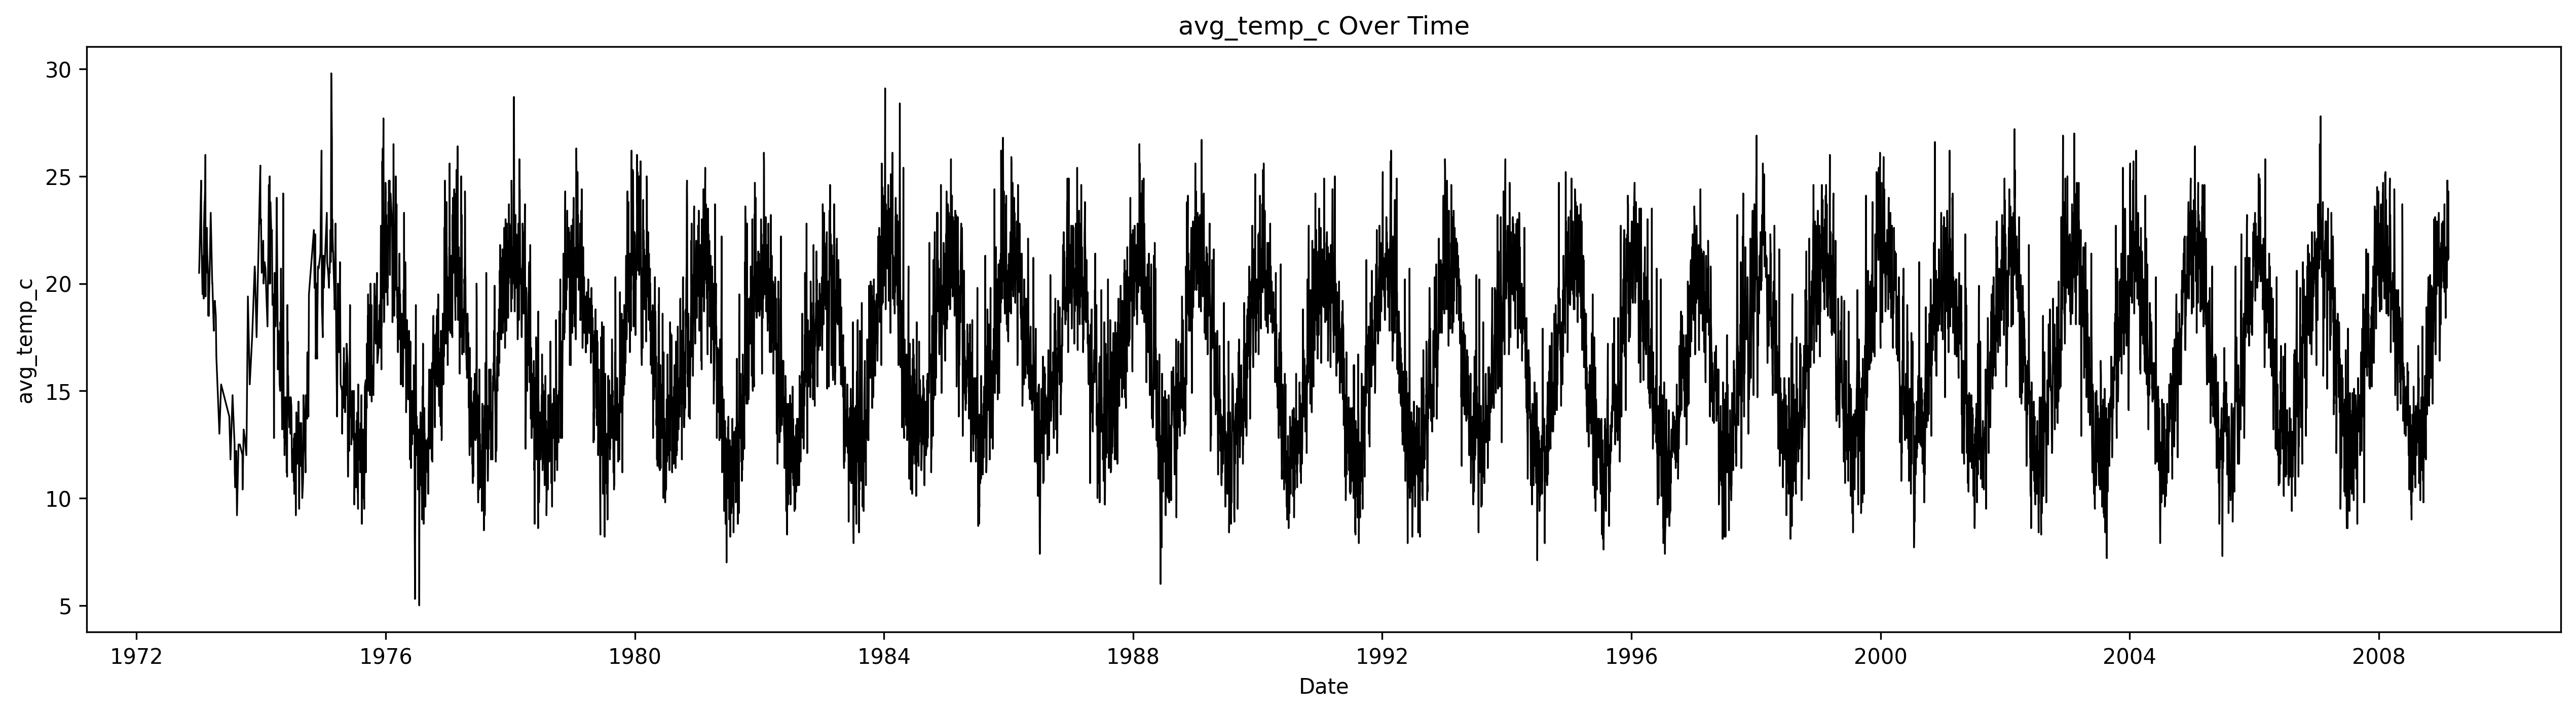
\includegraphics[width=1.0\linewidth]{../images/weather-over-time.pdf}
	\caption{Cape Town weather over time}
	\label{fig:cape-town-weather-time}
\end{figure}

The extreme cyclic nature made it very possible that the model would over-fit. The model did over-fit but surprisingly the validation performance was better then the test performance. Altering the learning rate, weight decay or drop-out did not mitigate this. The performance is relatively good considering it only uses one raw feature. If the previous day's weather was included as an additional feature this would probably greatly increase the performance. Other external data would also benefit performance. Here are the results from the cross-validation:

\begin{table}[htbp]
	\caption{Absolute difference between prediction and actual for best fold model (for unseen Cape Town weather data)}
	\resizebox{\columnwidth}{!}{
		\csvautobooktabular{../csv-descriptions/weather-rnn-results.csv}
	}
	\label{tab:weather-rnn-summary}
\end{table}

\begin{figure}[H] 
	\centering
	\includegraphics[width=1.0\linewidth]{../images/weather-elman-h32-actual-vs-predicted.pdf}
	\caption{Weather over time predictions (Jordan hidden layer size 32)}
	\label{fig:weather-predictions-elman}
\end{figure}

\subsubsection{Dataset 3: Air quality dataset}

\begin{table}[htbp]
	\caption{Absolute difference between prediction and actual for best fold model (for unseen Air quality data)}
	\resizebox{\columnwidth}{!}{
		\csvautobooktabular{../csv-descriptions/airquality-rnn-results.csv}
	}
	\label{tab:weather-rnn-summary}
\end{table}

\subsubsection{Dataset 3: Property price data set}

Here are the Elman RNN parameter choices for this dataset:

\begin{enumerate}[]
	\item Cross validation of 4 folds was used, due to large size of data set and computational restrictions.
	\item A robust scaler was used.
	\item Dropout of 0.2 was used.
	\item A batch size of 128 was used.
	\item Learning rate of 50, increased from 0.001 after noticing very slow convergence and difference in scale.
	\item A early stopping patience of 20.
	\item Model trained for 100 epochs.
\end{enumerate}

The Jordan model had equivalent parameters with a state layer of size 32.

Elman model initially over-fitted. Attempts were made to increase the drop-out and weight decay but this only improved the performance marginally.

\begin{figure}[H] 
	\centering
	\includegraphics[width=1.0\linewidth]{../images/House Elman (hidden size 32)-hs32-fold3.pdf}
	\caption{Showcasing of over-fitting of Elman model (hidden size 32)}
	\label{fig:overfit-elman-prop}
\end{figure}

\begin{table}[htbp]
	\caption{Absolute difference between prediction and actual for best fold model (for unseen House data)}
	\resizebox{\columnwidth}{!}{
		\csvautobooktabular{../csv-descriptions/house-rnn-results.csv}
	}
	\label{tab:house-rnn-summary}
\end{table}

From the results we can see the performance is not good and that more feature engineering would need to be done, potentially a moving average. The performance of the Elman model is better then the Jordan model.

\section{Conclusion}

The models are simply too complex to be trained with small datasets. The results seem to indicate that for smaller data sets the simpler models (Elman model) are preferred. Ideally you would not use a recurrent neural network at all for data sets of these sizes. It is also showcased that the pre-processing of the data set is very important for the models. With more advanced feature engineering techniques the model's performance would likely be better and the effect of feature engineering relates to the type of architecture used. 



\end{document}
